\documentclass[border=5mm,tikz,convert]{standalone}
\begin{document}
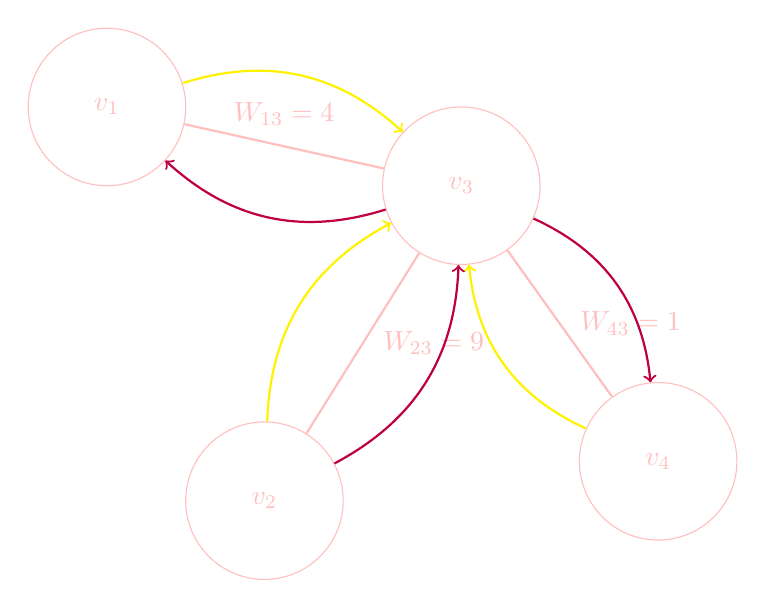
\begin{tikzpicture}[
nd/.style = {draw,circle,minimum size=2cm,pink},
edg/.style = {draw,thick,pink},
yel/.style = {draw,->,thick,yellow},
pur/.style = {draw,->,thick,purple}
]
  \node[nd] (v1) at (0,7) {$v_1$};
  \node[nd] (v2) at (2,2) {$v_2$};
  \node[nd] (v3) at (4.5,6) {$v_3$};
  \node[nd] (v4) at (7,2.5) {$v_4$};
  
  \path[edg] (v1)--(v3) node [midway, label=above:{$W_{13} = 4$}] {};
  \path[edg] (v2)--(v3) node [midway, label=right:{$W_{23} = 9$}] {};
  \path[edg] (v4)--(v3) node [midway, label=right:{$W_{43} = 1$}] {};
  
  \path[yel] (v1) edge [bend left] (v3);
  \path[yel] (v2) edge [bend left] (v3);
  \path[yel] (v4) edge [bend left] (v3);
  
  \path[pur] (v3) edge [bend left] (v1);
  \path[pur] (v2) edge [bend right] (v3);
  \path[pur] (v3) edge [bend left] (v4);
  
\end{tikzpicture}
\end{document}
